\documentclass[journal,10pt,twocolumn]{article}
\usepackage{graphicx}
\graphicspath{{./Figures/}}
\usepackage[margin=0.5in]{geometry}
\usepackage[cmex10]{amsmath}
\usepackage{amssymb}
\usepackage{array}
\usepackage{booktabs}
\title{Conic Assignment}
\def\myauthor{G Kumar}
\def\contact{kumargandhamaneni20016@gmail.com}
\def\mymodule{Future Wireless Communication (FWC)}
\date{}
\providecommand{\norm}[1]{\left\lVert#1\right\rVert}
\let\vec\mathbf
\newcommand{\myvec}[1]{\ensuremath{\begin{pmatrix}#1\end{pmatrix}}}
\newcommand{\mydet}[1]{\ensuremath{\begin{vmatrix}#1\end{vmatrix}}}
\providecommand{\brak}[1]{\ensuremath{\left(#1\right)}}
\usepackage{graphicx}
\graphicspath{{./images/}}
\usepackage[colorlinks,linkcolor={black},citecolor={blue!80!black},urlcolor={blue!80!black}]{hyperref}
\usepackage[parfill]{parskip}
\usepackage{lmodern}
\usepackage{tikz}
\usepackage{physics}
\usepackage{tabularx}
\usetikzlibrary{calc}
\usepackage{amsmath}
\usepackage{amssymb}
\renewcommand*\familydefault{\sfdefault}
\usepackage{watermark}
\usepackage{lipsum}
\usepackage{xcolor}
\usepackage{listings}
\usepackage{float}
\usepackage{titlesec}
\providecommand{\mtx}[1]{\mathbf{#1}}
\titlespacing{\subsection}{1pt}{\parskip}{3pt}
\titlespacing{\subsubsection}{0pt}{\parskip}{-\parskip}
\titlespacing{\paragraph}{0pt}{\parskip}{\parskip}
\newcommand{\figuremacro}[5]{
    \begin{figure}[#1]
        \centering
        \includegraphics[width=#5\columnwidth]{#2}
        \caption[#3]{\textbf{#3}#4}
        \label{fig:#2}
    \end{figure}
}
\lstset{
frame=single, 
breaklines=true,
columns=fullflexible
}
\thiswatermark{\centering \put(0,-105.0){
\includegraphics[scale=0.35]{iith}} }
\author{\myauthor\hspace{1em}\\\contact\\IITH\hspace{0.5em}-\hspace{0.5em}\mymodule}
\begin{document}
\maketitle
\section*{Problem}
The equation of the circle passing through the foci of the ellipse $\frac{x^2}{16}$+$\frac{y^2}{9}$=1,and having centre at (0,3) is
\section*{Solution}

\begin{figure}[h]
\centering
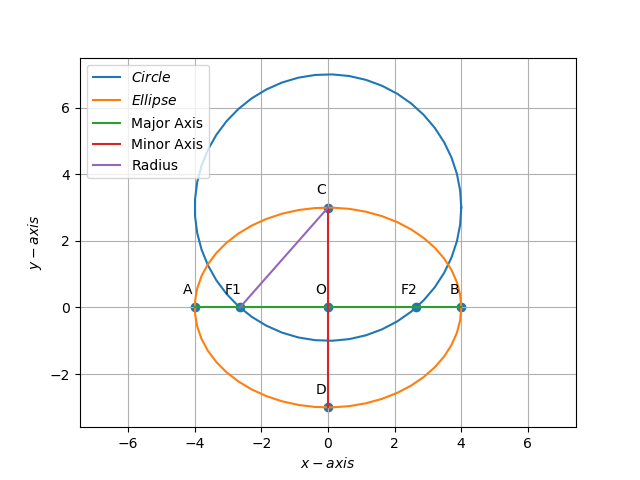
\includegraphics[width=1\columnwidth]{conic.png}
\caption{Ellpise with center O along with Circle C}
\label{fig:Ellipse}
\end{figure}

\subsection*{Step1}
Given, equation of an ellipse and centre of a circle passing through foci of the ellipse are,
\begin{align}
9x^2+16y^2-144=0,\hspace{1em}c=(0,3)
\end{align}
The equation of a conic with diretrix $\vec{n}^{\top}\vec{x} = c$, eccentricity e and Focus $\vec{F}$ is given by,
\begin{equation}
\vec{x}^{\top}\vec{V}\vec{x}+2\vec{u}^{\top}\vec{x}+f=0
\label{eq-1-}
\end{equation}
So,equation of ellipse in (1) can be written in form of (2) and centre in vector form as,
\begin{equation}
\vec{x}^{\top}\begin{pmatrix} 
	9 & 0 \\
	0 & 16 \\
	\end{pmatrix}\vec{x}+2\myvec{0&0}\vec{x}-144=0,\hspace{1em}\vec{C}=\myvec{0\\3}
\end{equation}
From this,
\begin{equation}
\vec{V} = \begin{pmatrix} 
	9 & 0 \\
	0 & 16 \\
	\end{pmatrix}, \hspace{4mm} \vec{u} = \myvec{0 \\ 0} \hspace{2mm} \& \hspace{2mm} f = -144
\label{eq-2-}
\end{equation}
Since $\vec{V}$ is symmetric,The eigenvalue decomposition of a symmetric matrix $\vec{V}$ is given by
\begin{equation}
\vec{P}^{\top}\vec{V}\vec{P} = \vec{D}   
\label{eq-3-}
\end{equation}
\begin{equation}
where, \vec{P}=\vec{I},\vec{D} = \begin{pmatrix} 
	\lambda_1 & 0 \\
	0 & \lambda_2 \\
	\end{pmatrix} 
\label{eq-4-}
\end{equation}
So, On solving $\eqref{eq-3-}$ using (6) and (4), we get
\begin{equation}
\vec{D} = \begin{pmatrix} 
	9 & 0 \\
	0 & 16 \\
	\end{pmatrix}
\label{eq-5-}
\end{equation}
This implies,
\begin{equation}
\lambda_1 = 9 \hspace{2mm} and \hspace{2mm} \lambda_2 = 16
\label{eq-6-}
\end{equation}
We have eccentricity,
\begin{equation}
e = \sqrt{1-\frac{\lambda_1}{\lambda_2}}
\label{eq-7-}
\end{equation}
from \eqref{eq-6-},
\begin{equation}
e = 0.6614
\label{eq-8-}
\end{equation}
For e $\neq$ 1, we have
\begin{equation}
c = \frac{e\vec{u}^{\top} \vec{n}\pm \sqrt{e^2\brak{\vec{u}^{\top}\vec{n}}^2 - \lambda_2 \brak{e^2-1}\brak{\norm{\vec{u}}^2-\lambda_2 f }}}{\lambda_2 e \brak{e^2-1}}
\label{eq-11-}
\end{equation}
Normal vector of diretrix $\vec{n}$ is given by
\begin{equation}
\vec{n} = \sqrt{\lambda_2}\vec{P_1}
\label{eq-9-}
\end{equation}
This gives,
\begin{equation}
\vec{n} = \myvec{4 \\ 0}
\label{eq-10-}
\end{equation}
On solving equation(11), using (4),(8),(10) and (13), we get,
\begin{equation}
c = \pm 24.1911
\label{eq-12-}
\end{equation}
Focii of a conic are given by,
\begin{equation}
\vec{F} = \frac{ce^2\vec{n}-\vec{u}}{\lambda_2}
\label{eq-13-}
\end{equation}
On solving, it yields,
\begin{equation}
\vec{F} = \myvec{\pm 2.6456\\0}
\label{eq-14-}
\end{equation}
Therefore, focii of the ellipse are,
\begin{equation}
\vec{F_1} = \myvec{-2.6456 \\ 0} \hspace{2mm} \& \hspace{2mm} \vec{F_2} = \myvec{2.6456 \\ 0}
\label{eq-15-}
\end{equation}
Let the equation of circle passing through the ellipse be,
\begin{equation}
\vec{x}^{\top}\vec{V}\vec{x}+2\vec{u_1}^{\top}\vec{x}+f_1=0
\label{eq-16-}
\end{equation}
\begin{equation}
where,\hspace{1em}\vec{V} = \vec{I}\hspace{1mm}and\hspace{2mm} \vec{u_1} = \myvec{0 \\ -3}
\end{equation}
Since circle is passing through $\vec{F_1}$,
\begin{equation}
\vec{F_1}^{\top}\vec{V}\vec{F_1}+2\vec{u_1}^{\top}\vec{F_1}+f_1=0 
\label{eq-18-}
\end{equation}
\begin{equation}
\myvec{-2.6456 & 0} \myvec{-2.6456 \\ 0} +  2\myvec{0 & -3}\myvec{-2.6456 \\ 0} +  f_1 = 0 
\end{equation}
\begin{gather*}
\implies f_1 = -6.99
\end{gather*}
Hence, Equation of the circle is given as,
\begin{equation}
\vec{x}^{\top}\vec{x}+2\myvec{0 & -3}\vec{x}-6.99=0
\label{eq-20-}
\end{equation}
\\
\textbf{Input parameters for this construction are:}
\begin{center}
    \setlength{\arrayrulewidth}{0.1mm}
	\setlength{\tabcolsep}{10pt}
	\renewcommand{\arraystretch}{1.5}
\begin{tabular}{|c|c|c|}
	\hline 
    \textbf{Symbol} & \textbf{Value} & \textbf{Description}\\ 		\hline
    $\vec{O}$ & $\myvec{0 \\ 0}$ & Center of Ellipse \\ \hline
    $\vec{A}$ & $\myvec{-4\\0}$ & Extreme point of major axis \\ \hline
    $\vec{B}$ & $\myvec{4\\0}$ & Extreme point of major axis \\ \hline
    $\vec{C}$ & $\myvec{0\\3}$ & Extreme point of minor axis and Center of circle (C) \\ \hline
    $\vec{D}$ & $\myvec{0\\-3}$ & Extreme point of minor axis \\ \hline
    $\vec{F_1}$ &$\myvec{-2.6456\\0}$ & Focus 1 of Ellipse \\ \hline
    $\vec{F_2}$ & $\myvec{2.6456\\0}$ & Focus 2 of Ellipse \\ \hline
\end{tabular}\\ \vspace{2mm}
Table 1: Parameter's Table
\end{center}

\end{document}